
%(BEGIN_QUESTION)
% Copyright 2005, Tony R. Kuphaldt, released under the Creative Commons Attribution License (v 1.0)
% This means you may do almost anything with this work of mine, so long as you give me proper credit

A student builds the following regulated AC-DC power supply circuit, but is dissatisfied with its performance:

$$\includegraphics[width=15.5cm]{i01473x01.eps}$$

The voltage regulation is not as good as the student hoped.  When loaded, the output voltage ``sags'' more than the student wants.  When the zener diode's voltage is measured under the same conditions (unloaded output, versus loaded output), its voltage is noted to sag a bit as well.  The student realizes that part of the problem here is loading of the zener diode through the transistor.  

\vskip 10pt

In an effort to improve the voltage regulation of this circuit, the student inserts an opamp ``voltage follower'' circuit between the zener diode and the transistor:

$$\includegraphics[width=15.5cm]{i01473x02.eps}$$

Now the zener diode is effectively isolated from the loading effects of the transistor, and by extension from the output load as well.  The opamp simply takes the zener's voltage and reproduces it at the transistor base, delivering as much current to the transistor as necessary without imposing any additional load on the zener diode.  While this modification does indeed improve the circuit's ability to hold a steady output voltage under changing load conditions, there is still room for improvement.  

\vskip 10pt

\filbreak

Another student looks at the modified circuit, and suggests one small change to dramatically improve the voltage regulation:

$$\includegraphics[width=15.5cm]{i01473x03.eps}$$

Now the output voltage holds steady at the zener diode's voltage with almost no ``sag'' under load!  The second student is pleased with the success, but the first student does not understand why this version of the circuit functions any better than previous version.  How would you explain this circuit's improved performance to the first student?  How is an understanding of negative feedback essential to being able to comprehend the operation of this circuit?

\vskip 10pt

One hint for explaining the opamp's new role is to relate it to the function of a {\it loop controller}, representing the input signals as {\it PV} and {\it SP}, and the output signal as the {\it Output}, with the transistor functioning like a {\it control valve}:

$$\includegraphics[width=15.5cm]{i01473x05.eps}$$

\vskip 20pt \vbox{\hrule \hbox{\strut \vrule{} {\bf Suggestions for Socratic discussion} \vrule} \hrule}

\begin{itemize}
\item{} Assuming a zener diode breakdown voltage of 5.0 volts, calculate the output voltage for each version of the power supply circuit.
\item{} Is the opamp ``loop controller'' functioning with {\it direct action} or {\it reverse action}?
\item{} Is the gain of the opamp ``loop controller'' significant to the regulation of power supply voltage?  In other words, will the voltage regulation be any better or worse if the internal (open-loop) voltage gain of the opamp were to change?
\item{} What would happen to this voltage regulator circuit if the resistor in series with the zener diode were to fail open?
\item{} What would happen to this voltage regulator circuit if the feedback wire connecting the opamp's inverting input terminal to the output terminal of the power supply were to fail open?
\item{} What would happen to this voltage regulator circuit if the transistor were to fail open from collector to emitter?
\end{itemize}

\underbar{file i01473}
%(END_QUESTION)





%(BEGIN_ANSWER)

With the relocated feedback connection, the opamp now ``senses'' the load voltage at the output terminals, and is able to correct for {\it any} voltage losses in the power transistor.  With the previous feedback connection (from the output terminal of the opamp), the opamp was only able to regulate voltage at the base of the transistor, not at the load itself.

%(END_ANSWER)





%(BEGIN_NOTES)

The last version of the voltage regulator circuit lets the opamp sense the actual output voltage, not just the drive to the transistor, allowing it to correct for any changes in transistor voltage drop.

\vskip 10pt

This is one of my favorite questions to ask students as they begin to learn how negative feedback works.  It is an excellent ``litmus test'' for comprehension of negative feedback: those students who understand how and why negative feedback works will immediately grasp the significance of the modified feedback connection; those who do not understand negative feedback will fail to grasp why this circuit works at all.  Spend as much time as you need discussing this circuit, because it holds the key to student understanding of a great many opamp circuits!

$$\includegraphics[width=15.5cm]{i01473x04.eps}$$

\vskip 20pt \vbox{\hrule \hbox{\strut \vrule{} {\bf Virtual Troubleshooting} \vrule} \hrule}

This question is a good candidate for a ``Virtual Troubleshooting'' exercise.  Presenting the diagram to students, you first imagine in your own mind a particular fault in the system.  Then, you present one or more symptoms of that fault (something noticeable by an operator or other user of the system).  Students then propose various diagnostic tests to perform on this system to identify the nature and location of the fault, as though they were technicians trying to troubleshoot the problem.  Your job is to tell them what the result(s) would be for each of the proposed diagnostic tests, documenting those results where all the students can see.

During and after the exercise, it is good to ask students follow-up questions such as:

\begin{itemize}
\item{} What does the result of the last diagnostic test tell you about the fault?
\item{} Suppose the results of the last diagnostic test were different.  What then would that result tell you about the fault?
\item{} Is the last diagnostic test the best one we could do?
\item{} What would be the ideal order of tests, to diagnose the problem in as few steps as possible?
\end{itemize}

%INDEX% Electronics review: opamp used in a voltage regulator circuit

%(END_NOTES)


